\section{System's perspective}
\subsection{Design}
When faced with initial task of refactoring the MiniTwit system, we agreed to choose a stack consisting of technologies at least one member of the group had experience with.
This enabled us to both have the advantage of working with something familiar but at the same time have the opportunity to learn something new. 

Our frontend is made using React with Typescript. When making the MiniTwit application we prioritized having the same functionality as the existing Flask application. As a result of this, the page setup and styling is identical to the original application.

We have used C\# for our back-end. The data access technology used is Entity Framework Core.

Our Database is a Managed Azure SQL database hosted on Azure. Originally we had Azure SQL Edge running in Docker but as the database data is important to save persistently we switched to Azure SQL running on a Microsoft Azure server. Azure allowed us to enable automatic tuning of the different tables that improved performance drastically (Indexation of tables). More on these topics in future sections.


\subsection{Architecture}
% \textcolor{red}{der er nogle af rapportudsnittene i helges slides som har skrevet at de bruger 4+1 men udelader logical og use case view, hvilket kunne være nice at gøre men det er nok lidt suspekt hvis vi gør det samme - 
% tror derfor at 3+1 er federe at bruge} \\
% \textcolor{blue}{overvej at opdele afsnittet i 3+1 eller 4+1, whatever vi mangler}

% This section aims to describe the architecture of our system, using the 3+1 model (KILDE!!!). \\

% The following deployment diagram illustrates the systems ?? view. 
% \begin{figure}[h]
%     \centering
%     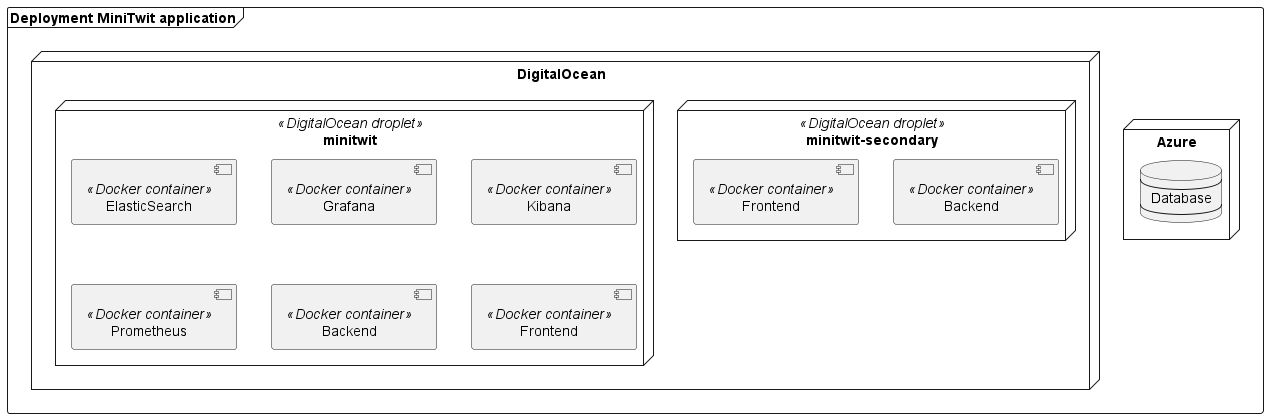
\includegraphics[width = \textwidth]{Images/deployment.png}
%     \caption{Deployment diagram illustrating the ?? view of our MiniTwit system}
%     \label{fig:DeploymentDiagram}
% \end{figure} \\
% As seen in figure 1, the system consists of a managed database on Microsoft's Azure platform as well as two separate droplets on DigitalOcean. The two droplets constitute our scaling setup which is described in depth in a future section. \\ The minitwit-secondary droplet runs the exact same images for frontend and backend.
% The most interesting parts to examine more deeply (from an architectural perspective) is the Docker containers for frontend and backend, as we wrote the code for those parts whereas the remaining 4 Docker containers (on the minitwit droplet) are just third party dependencies. \\
% Components??!?!?! 
This sections aims to describe the architecture of our system using Christensens 3+1 model \cite{architecturemodel} by showing
\begin{itemize}
    \item Requirements
    \item Module viewpoint 
    \item Component \& connectors viewpoint 
    \item Allocation / deployment viewpoint
\end{itemize}.
% Artikel https://citeseerx.ist.psu.edu/viewdoc/download?doi=10.1.1.555.5791&rep=rep1&type=pdf 
%Artikel der virker: https://pure.au.dk/portal/files/15565758/christensen-corry-marius-2007.pdf
%Slides: %https://baerbak.cs.au.dk/c/saip/slides/pdf/W2-1%20Views.pptx.pdf 
    
\subsubsection{Requirements}    
This section concerns the "+1" part of the 3+1 model i.e. the architectural requirements. \\
Though they referenced as "scenario-based" and "quality attribute-based" in the literature, this 
report will use the terms functional and non-functional requirements respectively. \\

\noindent
\textbf{Functional requirements}
\begin{enumerate}
    \item The system expose an API which adheres to the requirements of \cite{apispec} 
    \item Sumthing about minitwit website?
\end{enumerate} 

\noindent
\textbf{Non-functional requirements}
\begin{enumerate}
    \item C\# 
    \item React with Typescript 
    \item digitalocean
    \item docker
    \item performance, scalability, reliability
\end{enumerate}


    
    
\subsubsection{Module viewpoint}
Ting der skal være her ifølge 3+1 modellen: \\
- Elements: classes, packages, interfaces \\
- Relations: står i slides \\
- Mapping to UML: class diagrams (nok ikke relevant for os?) \\


This section attempts to describe how the functionality of our system is organized in code. 
At the highest level, the system is divided into backend and frontend.\\

The following package diagram gives a high-level overview of how the backend files are structured.
\begin{figure}[H]
 \centering
 \includegraphics[width = 0.4\textwidth]{Images/backend\_package\_overview.png}
 \caption{Backend Package overview}
 \label{fig:BackendPackageDiagram}
\end{figure}
\begin{itemize}
    \item \textbf{Domain:} contains the business entities of the system i.e. model and DTO classes representing users, tweets and followers.
    \item \textbf{DataAccess:} contains the class that handles sessions and communication with the database.
    \item \textbf{MiniTwitAPI:} houses the controller classes that make up both the public and internal APIs of the system, which are two separate units. 
\end{itemize}
A complete package diagram for the backend, including all relevant artifacts i.e., can be seen below. \\
No class diagrams will be shown, as this would not add anything interesting to the report. \\
\begin{figure}[H]
 \centering
 \includegraphics[width = 0.5\textwidth]{Images/backend\_complete\_package.png}
 \caption{Package diagram showing our backend artifacts}
 \label{fig:BackendCompletePackageDiagram}
\end{figure}
\textcolor{red}{skal dette diagram vise dependencies?}
\textcolor{red}{skal man gå dybere i det her lort?} \\

\newpage
The other interesting part of the program is the frontend, of which a package diagram is shown below.
Only the "src" package contains files of interest i.e. that we've written and not configuration or template files and as such the contents of "public", "nginx" and the root folder is not shown in the diagram. The artifacts represent the individual pages of the website as well as subcomponents, media, stylesheets and configuration-files that are React-specific. The naming of the pages reflects the naming from the original page structure provided.

\begin{figure}[H]
 \centering
 \includegraphics[width = \textwidth]{Images/package\_frontend.png}
 \caption{Package diagram of the frontend folder, only depicting the interesting parts}
 \label{fig:FrontendPackageDiagram}
\end{figure}


\subsubsection{Components \& connectors viewpoint}
\textcolor{red}{Denne sektion mangler tekst}\\
Dette viewpoint handler om: \\
- Components og deres "functional behaviour" / runtime \\
Jeg er ikke sikker på at diagrammet passer 100\% ind her eller at jeg forstår dette viewpoint helt. Det er dog meget vigtigt i følge ham der har lavet modellen. 


Hvad skal vi skrive til diagrammet? \\


The following diagram shows the six components i.e. Docker containers of our primary DigitalOcean droplet and how they interact with each other at runtime. The "MiniTwit backend" component contains two separate API subcomponents. The Docker container uses the same port to handle both API requests from the simulator and from the website but we've chosen to show it as two components in the diagram to enforce that they serve two different purposes.
\begin{figure}[H]
 \centering
 \includegraphics[width = \textwidth]{Images/all\_components.png}
 \caption{Component diagram of our primary DigitalOcean droplet}
 \label{fig:CompleteComponentDiagram}
\end{figure}


\subsubsection{Allocation / deployment viewpoint}
This section illustrates how elements of our system is mapped to infrastructure.


\textcolor{red}{Denne sektion mangler tekst} \\
Physical deployment: \\
- computers / execution environments \\
- Deployment units
- Communication links and dependencies

The following diagram .. 
\begin{figure}[H]
 \centering
 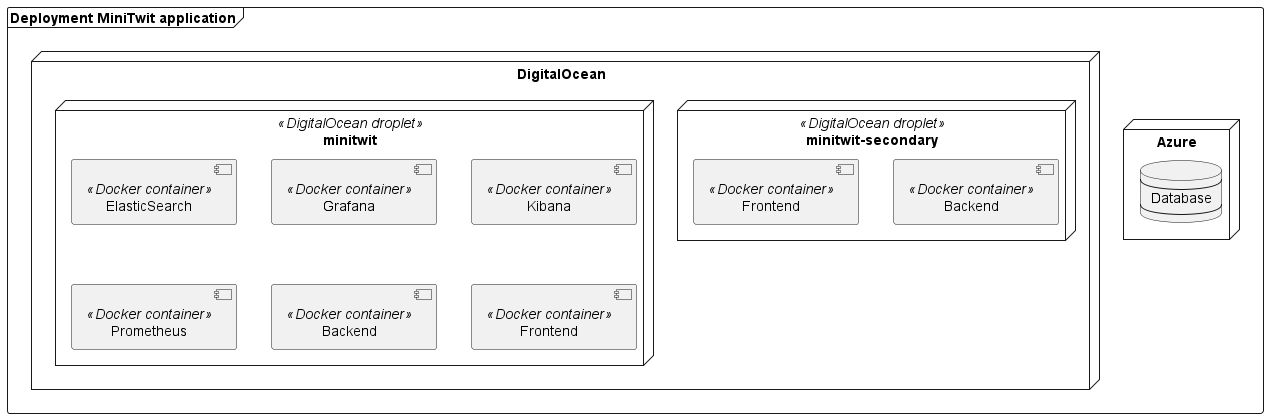
\includegraphics[width = \textwidth]{Images/deployment.png}
 \caption{Deployment diagram illustrating the overall deployment view of our MiniTwit system}
 \label{fig:DeploymentDiagram}
\end{figure}

\noindent
Both droplets are hosted on servers located in Frankfurt, Germany and they have the following specs: \\
\textbf{Primary} \\
- 1 vCPU
- 2 GB memory \\
- 50 GB disc space \\

\noindent
\textbf{Secondary} \\
- 1 vCPU \\
- 1 GB memory \\
- 25 GB disc space \\

They don't have the same specifications as they don't handle the same tasks but this will be elaborated in a later section.


\newpage
\subsection{Dependencies - technologies and tools}
% Der skal nok laves nogle diagrammer :) + der skal beskrivelser til hver \\
% Overvej om listen skal formatteres anderledes \\
% Skal vi inkludere de ting der blev brugt inden refactor også? \\

\textbf{Docker} is used for containerizing the system \\
\textbf{Python} is used for the old MiniTwit application. \\
\textbf{Bash} is used as terminal for the developers. \\
\textbf{C\# / ASP.NET CORE / dotnet} is used for our backend \\
\textbf{Ubuntu}, the OS that our droplets run on.\\
\textbf{React} our JavaScript library for building the website. \\
\textbf{Nginx} is a web server that runs React\\
\textbf{Keepalived} high-availability / scaling \\
\textbf{Docker-compose} handling multiple docker containers \\
\textbf{Dockerhub} storing docker images \\
\textbf{Typescript is used for React frontend} \\
\textbf{Git} version control \\
\textbf{Github} repository management \\
\textbf{Sonarcloud} static analysis \\
\textbf{DigitalOcean} provider of infrastructure \\
\textbf{Vagrant} \\
\textbf{CircleCI} continous integration pipeline \\
\textbf{Serilog} a library used for logging in the backend \\
\textbf{Prometheus} is used for system monitoring \\
\textbf{Grafana} is used to display monitoring information \\
\textbf{ElasticSearch} is used to aggregate the systems logs \\
\textbf{Kibana} is used to present the aggregated logs \\
\textbf{Azure SQL Edge} was used in a container in the first weeks of our project. As we wanted a separate permanent place to store the database we moved away from this.\\
\textbf{Azure SQL Database} is the Database system used for our MiniTwit application.\\
\textbf{Better Code Hub} provides static analysis of the code \\
\textbf{Microsoft Data Migration Assistant} is a tool that helped us migrate from Azure SQL Edge Database in a Droplet to the Azure SQL Database.\\
\textbf{SSMPT} is used to configure the mail server.\\
\textbf{MailUtils} is used to send a mail directly from a script using SSMTP server settings. Concretely this is an alert to notify us when Keepalived switches to another server than the Primary (when the primary dies)\\
\textbf{Gmail} is used as a central mailbox that forwards to our individual ITU mails.\\


\subsection{Important interactions of subsystems}
The most important interactions of subsystems in our MiniTwit applciation are the following 
\begin{itemize}
    \item HTTP communication between frontend and backend
    \item HTTP communication between backend and the simulator
    \item HTTP communication between backend and Prometheus
    \item ?? communication between Prometheus and Grafana
    \item HTTP communication between backend and ElasticSearch
    \item ?? communication between ElasticSearch and Kibana
\end{itemize}

The following sequence diagram shows the interaction between frontend and backend when a user posts a new message. \\
The flow of \textcolor{red}{most? all?} interactions between frontend and backend as well as between the backend and simulator follow the same flow, and as such we won't waste space on showing these. 

\begin{figure}[H]
 \centering
 \includegraphics[width = .5 \textwidth]{Images/frontend\_backend\_post\_messages\_sequence.png}
 \caption{Sequence diagram depicting the interaction between frontend and backend}
 \label{fig:SequenceDiagramPostMessage}
\end{figure}

The next sequence diagram shows an example of an interaction between the simulator, backend, ElasticSearch and database. In particular it depicts the sequence of logging and database calls that occur between a request to post a message being made and the response being returned to the simulator.

\begin{figure}[H]
 \centering
 \includegraphics[width = .9 \textwidth]{Images/sim\_backend\_elastic\_sequence.png}
 \caption{Sequence diagram depicting the interactions between the simulator, our simulator API, ElasticSearch and database that happen when the simulator posts a new message from a user}
 \label{fig:SequenceDiagramElasticBackendSim}
\end{figure}


\subsection{Current state of the system}
% \textcolor{red}{Giver nok bedst mening når vi er helt færdige med at arbejde - static analysis osv. kan bruges}
% \textcolor{red}{The API does not require any authorization. In the first week we implemented..}

In it's current form the system has a public API \\ 

Results from the static analysis tools X and Y are ... \\ 


\textcolor{red}{Hvis vi af en eller anden grund når noget af det her, så slet punkter} \\
The following are features and technologies that we would have liked to implement but did not.

\begin{enumerate}
    \item Infrastructure as code with Terraform
    \item Rolling updates 
    \item Automatic releases
    \item Running tests as part of CI (and terminating on test failure)
\end{enumerate}



\subsection{License compatibility}
The license used for this project is: \textbf{GNU GPL-3.0}. The list of licenses in the project can be seen in appendix \ref{ssec:licences}. According to license slide by Wheeler\cite{LicenseComp} the projects licence is compatible with the licenses: 
\begin{itemize}
    \item MIT
    \item Apache 2.0
    \item GNU GPL v3
    \item AGPL v2 
\end{itemize}
The license of the project should therefore be compatible with the licenses of its direct dependencies.